\chapter{Quantum Physics}

\begin{definition}
    A \vocab{photon} is a discrete packet (or quantum) of energy of electromagnetic radiation.
\end{definition}

\begin{proposition}
    The energy $E$ of a photon of electromagnetic radiation of frequency $f$ is given by \[E = hf = \frac{hc}{\l},\] where $h$ is the Planck constant.
\end{proposition}

\section{Photoelectric Effect}

\begin{definition}
    The \vocab{photoelectric effect} refers to the phenomenon that, when certain metal surfaces are illuminated by electromagnetic radiation, electrons are emitted from the surfaces.
\end{definition}

The electrons so emitted are called \vocab{photoelectrons}.

\subsection{Einstein's Photon Explanation}

If an electromagnetic radiation illuminates a metal surface and ejects an electron, wave theory predicts the following:
\begin{itemize}
    \item Electrons would be emitted at any frequency, provided the intensity of the radiation is high enough.
    \item The kinetic energy of the electron should depend on the intensity of the wave.
    \item Electrons would require some time to absorb incident radiation before they acquire enough kinetic energy to escape from the metal.
\end{itemize}

However, various observations of the photoelectric effect are not in accordance with the predictions of wave theory. These include:
\begin{itemize}
    \item No electron is emitted if the frequency of the radiation is below a certain threshold frequency $f_0$ even with very intense radiation. If the frequency of the radiation is above $f_0$, electrons are emitted even with low-intensity radiation.
    \item The maximum energy of the emitted electrons increases with the frequency of the radiation (above $f_0$) and is independent of the intensity of the radiation.
    \item There is negligible delay between illumination of the surface and emission of electrons.
\end{itemize}

Einstein suggested that, in its interaction with matter to release an electron, an electromagnetic radiation behaves as a stream of particle-like photons, each with energy proportional to the frequency of the radiation.
\begin{itemize}
    \item Each photon delivers a quantum of energy, $hf$, which could be absorbed by an electron immediately.
    \item Energy $\F$ is the minimum energy needed to free an electron from the surface.
    \begin{itemize}
        \item If $hf$ is less than $\F$, no electron is ejected. Higher intensity means more photons per second, but each photon is still unable to eject an electron.
        \item If $hf$ is greater than $\F$, the remainder is available to the electron as kinetic energy. Lower intensity means fewer photons per second, but each photon is still able to eject an electron.
    \end{itemize}
\end{itemize}

\begin{definition}
    The \vocab{work function energy} ($\F$) of a metal surface is the minimum energy (of a photon) required to release an electron from the surface.
\end{definition}

\begin{proposition}[Einstein's Photoelectric Equation]
    The photoelectric emission can be expressed as \[hf = \F + \frac12 m_e v_{\text{max}}^2,\] where $m_e$ is the mass of an electron and $v_{\text{max}}$ is the maximum speed of an emitted electron.
\end{proposition}

Note that even when the incident light is monochromatic, emitted electrons will have a range of values of kinetic energy up to the maximum value. This is because electrons not at the surface collide with other particles before reaching the surface, thus they require more energy to escape.

\begin{definition}
    The \vocab{threshold frequency} of a metal surface is the minimum frequency an electromagnetic radiation must have in order to cause photoelectric emission.
\end{definition}

\begin{proposition}
    The threshold frequency $f_0$ is related to the work function $\F$ by \[hf_0 = \F.\]
\end{proposition}
\begin{proof}
    If the radiation has frequency $f_0$, the emitted photoelectrons will have zero kinetic energy. Thus, $hf_0 = \F + 0 = \F$.
\end{proof}

\begin{corollary}
    An equivalent formulation for photoelectric emission is \[E_k = \frac12 m_e v_{\text{max}}^2 = hf - hf_0.\]
\end{corollary}
\begin{proof}
    From Einstein's photoelectric equation, \[hf = \F - \frac12 m_e v_{\text{max}}^2 = hf_0 - \frac12 m_e v_{\text{max}}^2 \implies \frac12 m_e v_{\text{max}}^2 = hf - hf_0.\]
\end{proof}

\subsection{Stopping Potential}

\begin{definition}
    One \vocab{electron volt} (eV) is the energy gained by an electron accelerated through a potential difference of one volt. \[1 \text{ eV} = e \times \bp{\text{1 V}} = \bp{1.60 \times 10^{-19} \text{ C}} \times \bp{1 \text{ V}} = 1.60 \times 10^{-19} \text{ J}.\]
\end{definition}

The electron volt is widely used to express the energy of photons and electrons because its magnitude is convenient in this area.

\begin{figure}[H]
    \centering
    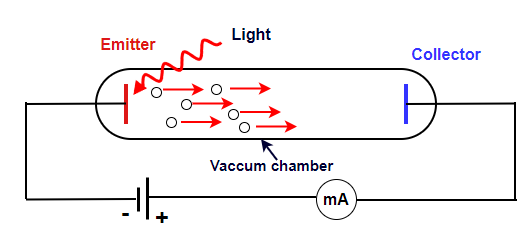
\includegraphics[scale=0.6]{media/Photoelectric Effect.png}
    \caption{Experimental set-up to observe the photoelectric effect.\protect\footnotemark}
\end{figure}
\footnotetext{Source: \url{https://iplts.com/physics/photoelectric-effect.php}}

The above figure shows an experimental set-up in which the photoelectric effect can be observed. An evacuated glass contains a metal electron (emitter, $E$) connected to the negative terminal of an e.m.f. source. Another metal electrode (collector, $C$) is connected to the positive terminal. $V$ is the potential of the collector relative to the emitter.

When monochromatic light, of frequency above $f_0$, shines on plate $E$, a current is detected by the ammeter, indicating a flow of photoelectrons across the plates $E$ and $C$.

If the electric field points towards the collector, as shown in the above figure, all the electrons are accelerated toward the collector and contribute to the photocurrent.

However, by reversing the electric field and adjusting its strength as in the figure below, we can determine the maximum kinetic energy of the emitted electrons by making $V$ negative enough so that the current $I$ stops. This occurs for $V = -V_S$, where $V_S$ is called the \vocab{stopping potential}.

\begin{proposition}
    At the stopping potential, \[eV_S = \frac12 m_e v_{\text{max}}^2 = hf - h_0.\]
\end{proposition}
\begin{proof}
    The most energetic electron leaves the emitter with kinetic energy $\frac12 m_e v_{\text{max}}^2$ and has zero kinetic energy at the collector. By the conservation of energy, $\D \text{KE} + \D \text{EPE} = 0$, so \[\bp{0 - \frac12 m_e v_{\text{max}}^2} + \bp{-e}(-V_S) = 0 \implies eV_S = \frac12 m_e v_{\text{max}}^2.\]
\end{proof}

\begin{figure}[H]
    \centering
    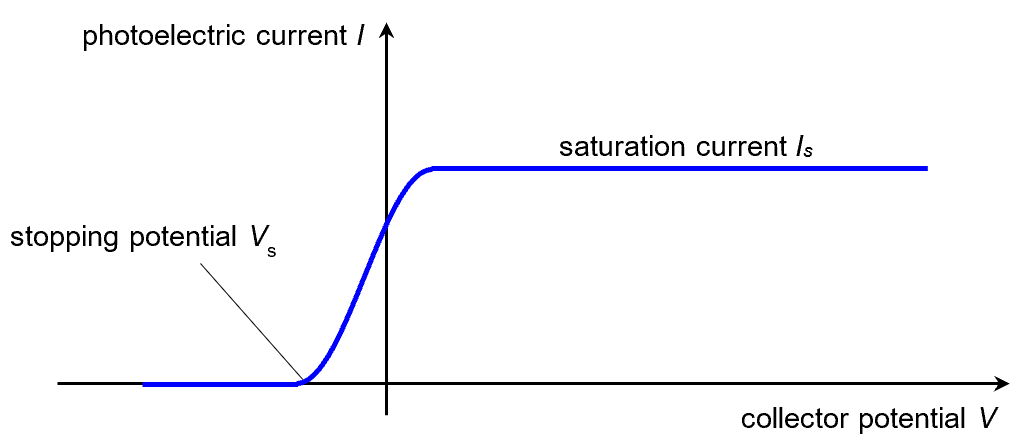
\includegraphics[scale=0.6]{media/Photoelectric Effect - IV Graph.png}
    \caption{A graph of the photoelectric current $I$ against the collector potential $V$.\protect\footnotemark}
\end{figure}
\footnotetext{Source: \url{https://xmphysics.com/2023/01/10/17-1-5-i-v-graph/}}

As $V$ increases from $-V_S$ towards 0 V, more photoelectrons reach the collector, hence the photocurrent increases. The current-voltage relationship in this region is approximately linear.

At 0 V, there is no accelerating or retarding potential. Hence, only photoelectrons with sufficient initial kinetic energy reach the collector.

As $V$ becomes positive, it accelerates all emitted photoelectrons towards the collector. The photocurrent rapidly increases until it reaches a saturation value. Beyond a certain positive voltage, any further increase in voltage will not increase the current.

The saturation current is determined by the intensity of the incident light (number of photons per second), as well as the quantum efficiency of the emitter (electrons emitted per incident photon).

\section{Wave Particle Duality}

\begin{definition}
    \vocab{Wave-particle duality} refers to the fact that matter behaves like waves in some situations and like particles in others.
\end{definition}

\begin{definition}
    The \vocab{de Broglie wavelength} ($\l$) is the wavelength associated with a particle that is moving, given by \[\l = \frac{h}{p} = \frac{h}{mv}.\]
\end{definition}

\begin{definition}
    The \vocab{de Broglie frequency} of a particle is related to its energy $E$ in exactly the same way as for a photon: \[E = hf.\]
\end{definition}

\begin{definition}
    The momentum $p$ associated with electromagnetic radiation of wavelength $\l$ is given by \[p = \frac{h}{\l} = \frac{hf}{c} = \frac{E}{c}.\]
\end{definition}

\section{Discrete Energy Levels}

\subsection{Energy Levels}

Atoms consist of a nucleus surrounded by electrons. In isolated atoms, these electrons occupy specific \vocab{energy levels} or \vocab{orbitals}, which are characterized by \vocab{principal quantum numbers} ($n$). The principal quantum number is a positive integer that primarily determines the energy of an electron in an atom. 

In quantum mechanics, electrons can only exist in certain allowed energy states, which are quantized (they have discrete values). The lowest energy state, corresponding to $n = 1$, is called the \vocab{ground state}. Any states above this $n > 1$ are referred to as \vocab{excited states}.

The Bohr model provides the simplest illustration of these discrete energy levels. In this model, electrons can only occupy specific circular orbits around the nucleus, each corresponding to a particular energy level and principal quantum number.

\begin{figure}[H]
    \centering
    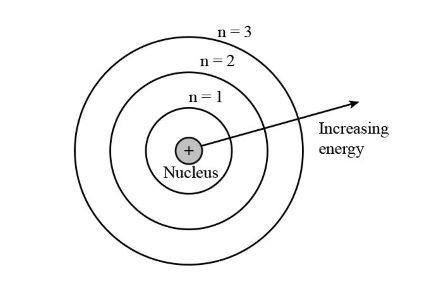
\includegraphics[scale=0.6]{media/Bohr Model.jpg}
    \caption{The Bohr model of an atom.}
\end{figure}

\subsection{Electron Transitions and Spectral Lines}

Electrons can move between these energy levels by absorbing or emitting energy. When an electron moves to a higher energy level (increasing $n$), it absorbs energy in a process called \vocab{excitation}. Electrons in excited states are inherently unstable and remain in these higher energy levels for only a very short time. Almost immediately, the electron falls to a lower energy level (decreasing $n$), releasing energy in a process called \vocab{de-excitation}. The energy changes in these transitions occur in the form of photons. The energy of each photon is equal to the energy difference between the levels involved in the transition.

\begin{figure}[H]
    \centering
    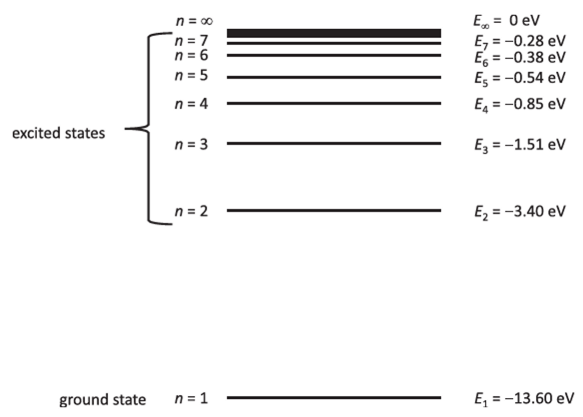
\includegraphics[scale=0.5]{media/Energy Level Diagram.png}
    \caption{The energy level diagram for a hydrogen atom. By convention, the energy of an electron at rest outside the atom is taken as zero.\protect\footnotemark}
\end{figure}
\footnotetext{Source: \url{https://ebrary.net/183922/mathematics/energy_levels_transitions}}

These electron transitions give rise to \vocab{spectral lines}. Each possible transition between energy levels produces a photon of specific energy, corresponding to light of a particular frequency of wavelength. The collection of these specific wavelengths form the atom's \vocab{spectrum}. When excited atoms emit photons, we observe an \vocab{emission spectrum}, which appears as bright lines on a dark background. Conversely, when atoms absorb specific wavelengths from white light, we see an \vocab{absorption spectrum}, appearing as dark lines in a continuous spectrum.

Each element has a unique set of energy levels, resulting in a distinct spectral pattern. This uniqueness allows for identification of elements based on their spectra.

\begin{figure}[H]
    \centering
    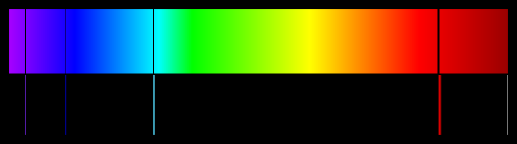
\includegraphics[scale=0.6]{media/Emission and Absorption Spectrum.png}
    \caption{The emission and absorption spectrum of hydrogen.\protect\footnotemark}
\end{figure}
\footnotetext{Source: \url{https://montessorimuddle.org/2012/02/01/emission-spectra-how-atoms-emit-and-absorb-light/}}

\subsection{X-Ray Spectra}

\vocab{X-rays} are electromagnetic radiation with wavelengths ranging from $10^{-12}$ m to $10^{-9}$ m. X-rays are ionizing radiation.

\subsubsection{Production of X-Rays}

X-ray tubes are devices which operate on high voltage in order to generate X-ray photons. A simplified diagram of an X-ray tube is shown below.

\begin{figure}[H]
    \centering
    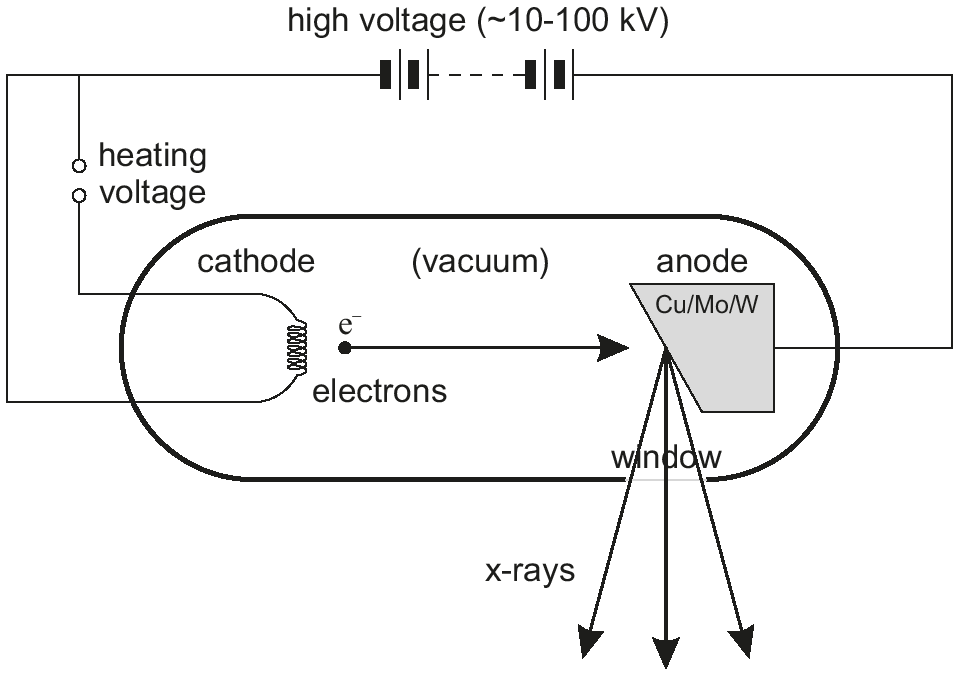
\includegraphics{media/X-Ray Tube.png}
    \caption{A diagram of an X-ray tube.\protect\footnotemark}
\end{figure}
\footnotetext{Source: \url{https://www.oreilly.com/library/view/biomedical-imaging/9783110423518/content/10_chapter03_4.xhtml}}

The filament is heated up by passing electric current through it, and emits electrons. The emitted electron gains kinetic energy given by \[E = e \D V,\] where $\D V$ is the potential difference in which the electron is accelerated across. When the electrons that are accelerated by the high voltage collide with a metal target, X-rays are emitted.

\subsubsection{X-Ray Spectrum}

A typical X-ray spectrum, a graph of intensity $I$ against wavelength $\l$ for the radiation emitted by an X-ray tube, is shown below.

\begin{figure}[H]
    \centering
    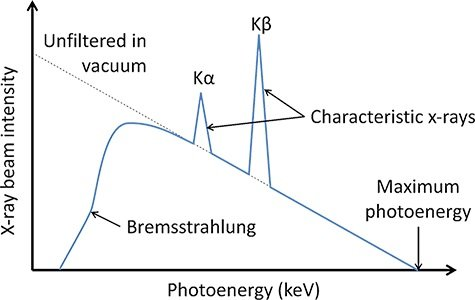
\includegraphics[scale=0.5]{media/X-Ray Spectrum.jpg}
    \caption{An X-ray spectrum.\protect\footnotemark}
\end{figure}
\footnotetext{Source: \url{https://physicsopenlab.org/2018/02/13/x-ray-emission/}}

It has a continuous broad spectrum called \vocab{bremsstrahlung} (lit. braking radiation) and a series of sharp peaks called \vocab{characteristic X-rays}.

The bremsstrahlung are emitted as a result of sudden deceleration of the electrons when they collide with the dense metal target. A wide range of decelerations give rise to photons with a wide range of energies and so a continuous spectrum.

The bremsstrahlung cuts off rapidly at a minimum wavelength $\l_{\text{min}}$ which is independent of the target metal, but depends on the maximum energy of the electrons, which in turn depends on the accelerating potential difference $\D V$. A higher $\D V$ will produce a shorter cut-off wavelength $\l_{\text{min}}$.

The characteristic X-rays are emitted when electrons transit from higher to lower energy levels in the target atoms. The peaks correspond to the emission spectrum of the target atom. The accelerating potential difference $\D V$ has to exceed a certain value, usually called the threshold voltage, for the characteristic X-rays to be observed.

\section{Heisenberg's Uncertainty Principle}

\begin{principle}[Heisenberg's Uncertainty Principle]
    For a particle, the product of the uncertainties in position ($\D x$) and momentum ($\D p$) in the same direction cannot be smaller than the Planck constant $h$: \[\D x \D p \geq h.\]
\end{principle}

This principle implies that it is impossible to simultaneously determine both the exact position and exact momentum of a particle.